\documentclass[bachelor, och, coursework]{SCWorks}
% параметр - тип обучения - одно из значений:
%    spec     - специальность
%    bachelor - бакалавриат (по умолчанию)
%    master   - магистратура
% параметр - форма обучения - одно из значений:
%    och   - очное (по умолчанию)
%    zaoch - заочное
% параметр - тип работы - одно из значений:
%    referat    - реферат
%    coursework - курсовая работа (по умолчанию)
%    diploma    - дипломная работа
%    pract      - отчет по практике
% параметр - включение шрифта
%    times    - включение шрифта Times New Roman (если установлен)
%               по умолчанию выключен
\usepackage{subfigure}
\usepackage{tikz,pgfplots}
\pgfplotsset{compat=1.5}
\usepackage{float}

%\usepackage{titlesec}
\setcounter{secnumdepth}{4}
%\titleformat{\paragraph}
%{\normalfont\normalsize}{\theparagraph}{1em}{}
%\titlespacing*{\paragraph}
%{35.5pt}{3.25ex plus 1ex minus .2ex}{1.5ex plus .2ex}

\titleformat{\paragraph}[block]
{\hspace{1.25cm}\normalfont}
{\theparagraph}{1ex}{}
\titlespacing{\paragraph}
{0cm}{2ex plus 1ex minus .2ex}{.4ex plus.2ex}

% --------------------------------------------------------------------------%


\usepackage[T2A]{fontenc}
\usepackage[utf8]{inputenc}
\usepackage{graphicx}
\graphicspath{ {./images/} }
\usepackage{tempora}

\usepackage[sort,compress]{cite}
\usepackage{amsmath}
\usepackage{amssymb}
\usepackage{amsthm}
\usepackage{fancyvrb}
\usepackage{listings}
\usepackage{listingsutf8}
\usepackage{longtable}
\usepackage{array}
\usepackage[english,russian]{babel}

% \usepackage[colorlinks=true]{hyperref}
\usepackage{url}

\usepackage{underscore}
\usepackage{setspace}
\usepackage{indentfirst} 
\usepackage{mathtools}
\usepackage{amsfonts}
\usepackage{enumitem}
\usepackage{tikz}
\usepackage{minted}

\newcommand{\eqdef}{\stackrel {\rm def}{=}}
\newcommand{\specialcell}[2][c]{%
\begin{tabular}[#1]{@{}c@{}}#2\end{tabular}}

\renewcommand\theFancyVerbLine{\small\arabic{FancyVerbLine}}

\newtheorem{lem}{Лемма}

\begin{document}

% Кафедра (в родительном падеже)
\chair{теоретических основ компьютерной безопасности и криптографии}

% Тема работы
\title{Генерация текстового описания к изображению с помощью нейронной сети}

% Курс
\course{3}

% Группа
\group{331}

% Факультет (в родительном падеже) (по умолчанию "факультета КНиИТ")
\department{факультета КНиИТ}

% Специальность/направление код - наименование
%\napravlenie{09.03.04 "--- Программная инженерия}
%\napravlenie{010500 "--- Математическое обеспечение и администрирование информационных систем}
%\napravlenie{230100 "--- Информатика и вычислительная техника}
%\napravlenie{231000 "--- Программная инженерия}
\napravlenie{100501 "--- Компьютерная безопасность}

% Для студентки. Для работы студента следующая команда не нужна.
% \studenttitle{Студентки}

% Фамилия, имя, отчество в родительном падеже
\author{Улитина Ивана Владимировича}

% Заведующий кафедрой
\chtitle{} % степень, звание
\chname{Абросимов М. Б.}

%Научный руководитель (для реферата преподаватель проверяющий работу)
\satitle{доцент} %должность, степень, звание
\saname{Слеповичев И. И.}

% Руководитель практики от организации (только для практики,
% для остальных типов работ не используется)
% \patitle{к.ф.-м.н.}
% \paname{С.~В.~Миронов}

% Семестр (только для практики, для остальных
% типов работ не используется)
%\term{8}

% Наименование практики (только для практики, для остальных
% типов работ не используется)
%\practtype{преддипломная}

% Продолжительность практики (количество недель) (только для практики,
% для остальных типов работ не используется)
%\duration{4}

% Даты начала и окончания практики (только для практики, для остальных
% типов работ не используется)
%\practStart{30.04.2019}
%\practFinish{27.05.2019}

% Год выполнения отчета
\date{2022}

\maketitle

% Включение нумерации рисунков, формул и таблиц по разделам
% (по умолчанию - нумерация сквозная)
% (допускается оба вида нумерации)
% \secNumbering

%-------------------------------------------------------------------------------------------

\tableofcontents

\intro

    Последнее десятилетие имплементации алгоритмов искусственного интеллекта раз
    за разом поражали людей своими способностями решать задачи, считавшиеся до
    этого выполнимыми исключительно человеком. И с каждым годом темп развития
    этой сферы информационных технологий многократно увеличивался, всё сильнее
    поражая людей обширностью потенциала и возможностей использования глубокого
    обучения в повседневной жизни, которая постепенно преображалась в силу
    движения прогресса. В современном мире так много приложений нейросетевых
    алгоритмов в самых различных отраслях человеческой жизнедеятельности, что
    всё чаще человек использует ИИ, иногда даже не подозревая об этом. От
    нахождения кратчайшего пути из дома до аэропорта и прогнозирования погоды по
    параметрам воздуха и вплоть до удовлетворения банковских услуг пользователя
    с помощью автоответчика "--- всё это напрямую говорит об удивительном
    множестве возможностей использования искусственного интеллекта, которое
    постоянно расширяется.
    
    Среди разделов глубокого обучения, использование которых ввергает людей в
    восхищение перед возможностями ИИ, следует выделить \textbf{NLP} и
    \textbf{Computer Vision}. В данной работе пойдёт речь именно о такой
    совокупности нейросетей, которая будет осуществлять обработку изображения
    таким образом, чтобы ко входному для алгоритма рисунку генерировалось
    текстовое описание. Чаще всего, в англоязычных ресурсах данная задача
    называется \textbf{Image Captioning}, и реализации её решения являются
    прикладной технологией для самых различных нужд \cite{neur}.

    % Вероятно, будет полезно в тех случаях, когда чаще всего используется
    % текст, и с его помощью вы можете вывести/генерировать текст из
    % изображений. Например, использовать информацию непосредственно из любого
    % конкретного изображения в текстовом формате автоматически. В настоящее
    % время существует множество приложений НЛП, которые извлекают
    % информацию/резюме из заданных текстовых данных, эссе и т. д. Те же
    % преимущества могут быть получены людьми, которые выиграют от
    % автоматизированного анализа изображений. Слегка (не очень) долгосрочным
    % вариантом использования, безусловно, было бы объяснение того, что
    % происходит в видео, кадр за кадром. Послужит огромным подспорьем для
    % слабовидящих людей. В этом пространстве можно разработать множество
    % приложений. Социальные сети. Такие платформы, как Facebook, могут делать
    % выводы непосредственно из изображения, где вы находитесь (пляж, кафе и т.
    % д.), что вы носите (цвет) и, что более важно, что вы делаете (в каком-то
    % смысле). Посмотрите пример, чтобы лучше понять его.

\defabbr

    Перед анализом теоретической составляющей глубокого обучения и архитектур
    нейронных сетей, которые осуществляют генерацию текстового описания к
    входному для алгоритма изображению, стоит ввести ряд терминов и определений,
    являющихся основой для понимания работы алгоритма генерации \cite{Gud}.

    \textit{Искусственный интеллект} (англ. Artificial Intelligence) "---
    технология создания алгоритмов, лежащих в основе проектирования
    интеллектуальных машин и программ, способных имитировать деятельность
    человека.

    \textit{Нейронная сеть (нейросеть)} (англ. Neural Network) "---
    математическая модель, чаще всего имеющая программную интерпретацию, сутью
    которой является реализация деятельности, похожей на деятельность
    биологических нейронных сетей. Нейронная сеть используется при создании
    какого-либо из алгоритмов искусственного интеллекта и состоит из
    совокупности нейронов, соединенных между собой связями. 

    \textit{Признак} (англ. Feature) "--- каждый отдельный элемент информации,
    включаемый в представление о каком-либо анализируемом объекте.

    \textit{Машинное обучение} (англ. Machine Learning) "--- область науки об
    искусственном интеллекте, которая изучает способы создания алгоритмов,
    которые могут обучаться (развиваться).

    \textit{Глубокое обучение} (англ. Deep Learning) "--- частный случай
    машинного обучения, который представляет из себя методы машинного обучения,
    основанные на обучении представлений. Осуществляет получение представлений
    путем их выражения через более простые представления, а формирование
    последних, в свою очередь, реализуется через ещё более простые
    представления, и так далее.

    \textit{Компьютерное зрение} (англ. Computer Vision) "--- область науки об
    искусственном интеллекте, использующая методы машинного и глубокого обучения
    для решения задач распознавания, классификации, мониторинга с помощью
    получения необходимой информации из изображения.

    \textit{Обработка естественного языка} (англ. Natural Language Processing,
    NLP) "--- направление развития ИИ и математической лингвистики, которое
    изучает проблемы синтеза и компьютерного анализа текстов на естественных
    языках. Говоря об искусственном интеллекте, под анализом подразумевается
    понимание языка, а под синтезом "--- генерация грамотного с точки зрения
    языковых норм текста.

    \textit{Текстовое описание к изображению} (англ. Image Captioning) "--- это
    задача описания содержания изображения словами естественного языка. Принцип
    решения лежит на пересечении таких разделов глубокого обучения как
    компьютерного зрения и обработки естественного языка. В большинстве систем
    генерации текстовых описаний к изображениям используется структура
    кодировщик-декодер, в которой входное изображение кодируется в промежуточное
    представление информации о содержимом изображения, а затем декодируется в
    описательную текстовую последовательность.

\section{Теоретическая часть}

    \subsection{Сверточная нейронная сеть}

        % Принцип работы
        Искусственные нейронные сети или ИНС (англ. Artificial Neural Network
        или ANN) "--- это системы вычислительной обработки, принцип работы
        которых в значительной степени основан на том, как работают
        биологические нервные системы (в частности, человеческий мозг). ИНС в
        основном состоят из большого количества взаимосвязанных вычислительных
        узлов (называемых нейронами), работа которых определяется соединениями
        со слоями, содержащими другие нейроны. В итоге совокупность вычислений,
        производимых этими нейронами, осуществляет процесс обучения, который
        заключается в минимизации ошибки окончательного вывода нейросети (т.е.
        результата её работы).
        
        Сверточные нейронные сети (англ. Convolutional Neural Network, CNN)
        аналогичны традиционным ANN в том, что они состоят из нейронов, которые
        самооптимизируются посредством обучения. Принцип, при котором каждый
        нейрон получает входные данные и выполняет операцию (например, скалярное
        произведение, за которым следует применение нелинейной функции) "--- это
        основа бесчисленных вариантов реализаций ИНС. Организовывая процесс
        преобразования входных необработанных векторов изображений в некоторый
        окончательный результат (будь то обработка изображения, классификация
        изображения или генерация текстовой подписи), вся нейросеть по-прежнему
        будет представлять собой функции преобразования весов-коэффициентов.
        Последний слой будет содержать функцию потерь, определяемую классом
        решаемой задачи, и все обычные принципы организации архитектуры модели,
        разработанные для традиционных ИНС, также могут быть применимы и в
        работе со сверточными нейросетями \cite{cnn1}. 

        Принципиальное отличие обычной нейронной сети от сверточной является
        наличие в последней специального ''сверточного'' слоя, который применяет
        к входным весам математическую операцию свертки. Термин свертка
        относится к математической комбинации двух функций для получения третьей
        функции. В случае CNN свертка выполняется для входных данных с
        использованием фильтра или ядра (эти термины взаимозаменяемы), чтобы
        затем создать карту признаков (англ. feature map). Выполнение свертки
        осуществляется перемещением фильтра по минорам входной матрицы. Для
        каждого минора определенного размера выполняется матричное умножение с
        соответствующим ему фильтром и суммируется результат на карте признаков. 

        \begin{figure}[H]
            \centering
            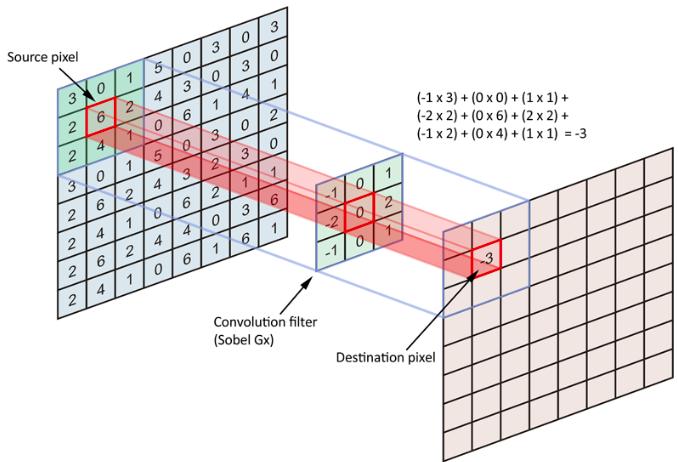
\includegraphics[width=0.8\textwidth]{pics/convolute.png}
            \caption{Операция свёртки}
        \end{figure}

        Операции свертки выполняются на входной матрице, где каждая операция
        использует определенный фильтр. Результатом итераций математической
        процедуры являются различные карты признаков. В качестве шага,
        завершающего операцию, берутся все эти карты признаков и объединяются
        вместе в качестве конечного результата сверточного слоя.

        % Область применения
        Сверточная нейронная сеть "--- это алгоритм глубокого обучения, который
        применяется для обработки данных с сеточной топологией. Один из примеров
        такого вида данных "--- временные ряды, которые представимы в виде
        одномерной сетки примеров, выбираемых через регулярные промежутки
        времени (англ. timestamp). Вторым, более актуальным для этой работы
        примером, являются изображения, которые можно интерпретировать как
        двумерную сетку пикселей \cite{cnn2}.

        Популярность использования такого вида нейросетей при работе с
        изображениями обусловлена их отличительными положительными чертами.
        Сверточные нейронные сети обеспечивают частичную устойчивость к
        изменениям масштаба, смещениям, поворотам, смене ракурса и прочим
        искажениям картинки. Сверточные нейронные сети объединяют три
        архитектурных идеи, для обеспечения инвариантности к масштабируемости,
        вращению и другим пространственным деформациям:

        \begin{enumerate}
            \item
                локальные рецепторные поля (обеспечивают локальную двумерную
                связность нейронов);
            \item
                общие синаптические коэффициенты (обеспечивают детектирование
                некоторых черт в любом месте изображения и уменьшают общее число
                весовых коэффициентов);
            \item
                иерархическая организация с пространственными подвыборками.
        \end{enumerate}

    \subsection{Рекуррентная нейронная сеть и LSTM}

        % Принцип работы
        Рекуррентная нейронная сеть или РНС (англ. Recurrent Neural Network,
        RNN) "--- это тип искусственной нейронной сети, которая обрабатывает
        последовательности данных и временные ряды. Подобно нейронным сетям с
        прямой связью (англ. Feedforward Neural Network, FNN) и CNN,
        рекуррентные нейронные сети используют обучающие данные для изменения
        своих весов. Основным отличием от других видов сетей является
        ''память'', суть которой в том, что в процессе обработки входной
        информации особым текущим слоем в RNN, используются входные параметры к
        некоторым предыдущим слоям сети (таким образом влияя на результат работы
        текущего слоя сети). В то время как традиционные глубокие нейронные сети
        предполагают, что входные и выходные данные слоев независимы друг от
        друга, выходы рекуррентных нейронных сетей зависят от предшествующих
        элементов внутри последовательности этих слоев. Хотя будущие
        преобразования также могут быть полезны для определения результата
        данной последовательности, однонаправленные рекуррентные нейронные сети
        не могут учитывать эти преобразования в своих прогнозах \cite{rnn1}.

        \begin{figure}[H]
            \centering
            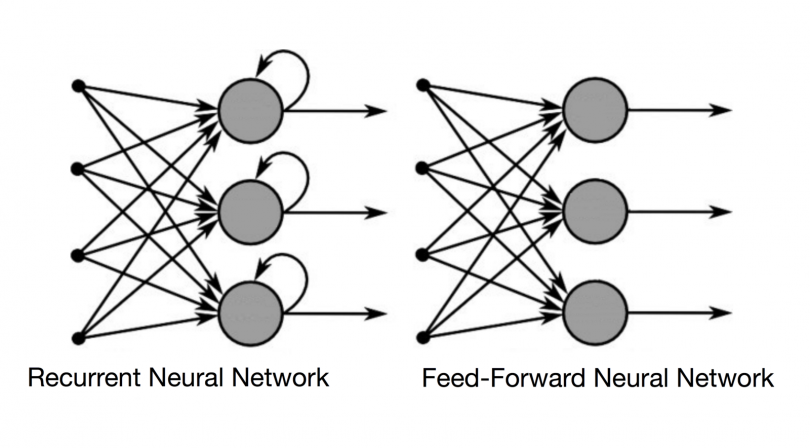
\includegraphics[width=0.8\textwidth]{pics/rnn-vs-fnn.png}
            \caption{Абстрактное сравнение архитектур FNN и RNN}
        \end{figure}

        Однако при использовании первых архитектур RNN возникала проблема потери
        способности связывать информацию в силу уменьшения влияния аргументов
        слоев сети на текущий обрабатываемый слой по мере увеличения
        ''расстояния'' между слоем, для которого были изначально предназначены
        аргументы, и текущим слоем. Уменьшение влияния выражается через проблему
        исчезающего градиента (англ. Vanishing gradient problem), которая
        возникает в процессе обучения ANN с помощью методов, основанных на
        градиентном спуске (англ. Gradient Descent) и методе обратного
        распространения ошибки (англ. Backpropagation). В этих способах
        обучения, на протяжении всей итерации обучения или эпохи, каждый из
        весов нейросети обновляется пропорционально частной производной функции
        ошибки от текущего веса. Время от времени значение градиента может
        становиться бесконечно малым, что препятствует обновлению значения веса.
        На практике, в силу отсутствия возможности сохранения качества передачи
        параметров между слоями, была представлена реализация модификации
        рекуррентной нейросети, которая способна к обучению долговременным
        зависимостям. Название такого подкласса RNN "--- сеть с долгой
        краткосрочной памятью (англ. Long Short-Term Memory, LSTM).

        Решение с помощью LSTM использует карусель с постоянными ошибками (англ.
        Constant Error Carousel, CEC), которые обеспечивают постоянный поток
        ошибок (необходимый для хранения значений ошибки для дальнейшего
        обучения модели) в специальных ячейках. Доступ к ячейкам (и их
        применение) осуществляется мультипликативными блоками ворот (англ. gate
        units), которые учатся своевременно предоставлять этот доступ. CEC
        являются центральной функцией LSTM, где осуществляется хранение
        краткосрочной памяти в течении длительных периодов времени. В ходе
        выполнения обработки соединений между другими блоками сети LSTM может
        также возникнуть конфликт обновления веса. Входные соединения некоторого
        нейрона $u$ могут конфликтовать в процессе обновления веса по причине
        того, что один и тот же вес может как использоваться для хранения
        некоторого входного значения, так и не использоваться. Для взвешенных
        выходов соединений, идущих от нейрона $u$, одинаковые веса могут вернуть
        содержимое $u$ и сделать поток вывода ошибки в другие нейроны сети
        некорректным. Эту проблему решает расширение CEC входными и выходными
        блоками ворот, которые соединены с входным слоем сети и с другими
        ячейками памяти, что ведет к формированию особого блока LSTM,
        называемого блоком памяти (англ. Memory Block) \cite{lstm1}.

        \begin{figure}[H]
            \centering
            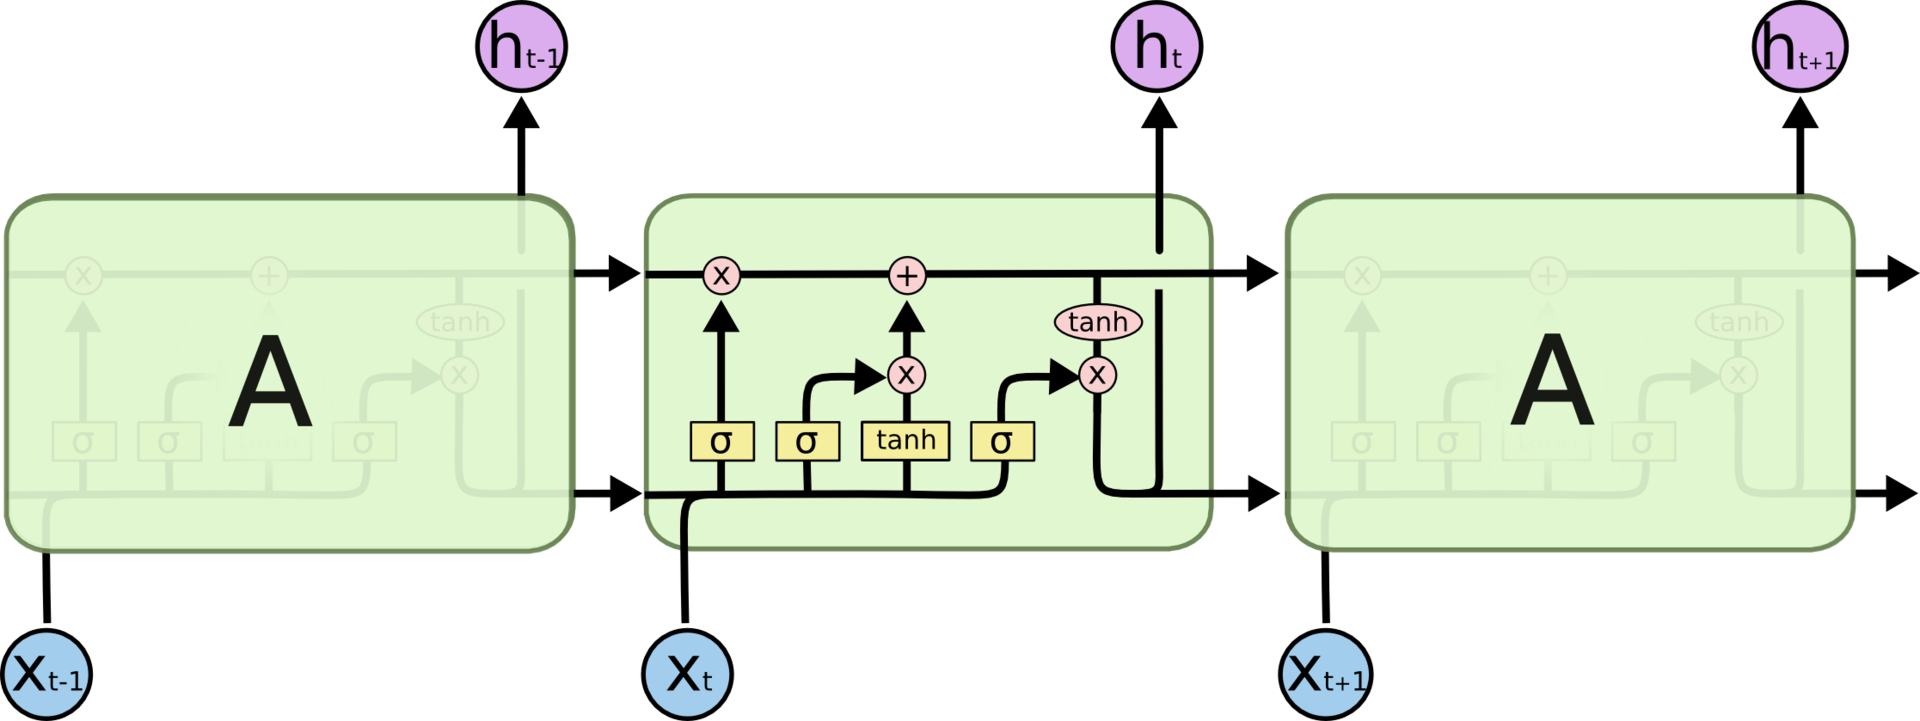
\includegraphics[width=0.8\textwidth]{pics/lstm.png}
            \caption{Схема содержимого модуля LSTM-сети}
        \end{figure}

        % Область применения
        РНС "--- это такой тип архитектуры нейронной сети, который
        преимущественно используется для нахождения закономерностей и шаблонов
        (англ. pattern) в последовательностях данных. Такими данными могут быть
        рукописи, представления геномов, текст или числовые временные ряды,
        часто используемые в рамках корпоративных задач машинного обучения
        (например, даны показатели курса некоторой акции или валюты, и требуется
        предсказать значение стоимости акции в следующий момент времени, или
        представлены значения сенсоров в течении некоторого временного
        промежутка и необходимо осуществить классификацию поведения этого
        сенсора). В общем смысле, RNN применяются в моделировании языка (англ.
        Language Modelling) и генерация текста, распознавании речи, генерации
        описания к изображениям (не только текстового, но и по возможным другим
        параметрам) или маркировке видео (англ. Video Tagging) \cite{rnn2}.
        
        В свою очередь, LSTM-сети (как подкласс сетей RNN) могут применяться в
        тех же сферах, что и обычные рекуррентные сети. В 2012 году модификация
        LSTM была применена для обнаружения ключевых слов и распознавания
        различных видов содержимого рукописных документов (такие как текст,
        формула, диаграмма и рисунок). Примерно в тот же период времени с
        помощью сетей с долгой краткосрочной памятью осуществлялась
        классификация изображений высокого разрешения из базы данных ImageNet,
        результаты которой были значительно лучше предыдущих (без использования
        LSTM). В 2015 году разновидность этого класса нейросети с использованием
        фреймворка Sequence-to-Sequence была успешно обучена для создания
        предложений на простом английском языке, описывающих изображения. Также
        в 2015 году LSTM была объединена с глубоким иерархическим экстрактором
        визуальных признаков и применена к решению задач интерпретации и
        классификации изображений, таких как определение некоторого активного
        действия на картинке и генерация описания изображения/видео
        \cite{lstm2}.

    \subsection{Метрики оценки качества обучения}

        Как известно, машинное обучение "--- это такая область информационных
        технологий, которая рассматривает процессы обучения нейросетей в целях
        достижения высокоуровневого познания и проведения человекоподобного
        анализа различных задач. Поскольку ML подразумевает использование данных
        в процессе обучения, это прекрасно вписывается в повседневную
        жизнедеятельность человечества, так же как и в комплексные и
        междисциплинарные деятельности. С ростом популярности инструментов
        машинного обучения, подразумевающих коммерциализацию, открытый исходный
        код или ориентацию на конечного пользователя, при использовании ИИ в той
        или иной задаче всегда возникает закономерный вопрос "--- какие факторы
        определяют хорошую модель? Правильный ответ на этот вопрос зависит от
        совокупности факторов, которые для каждой определенной модели могут
        определяться по-своему \cite{metrics1}.

        Одним из факторов, определяющих, каким образом следует оценивать модель,
        является то, какой тип задач решается этой моделью, среди которых можно
        выделить самые популярные, а именно:
        
        \begin{enumerate}
            \item
                Регрессия "--- прогноз на основе выборке объектов с различными
                значениями конечного числа признаков. В качестве результата
                модель для определенного набора характеристик, определяющихся
                этими признаками, должна вернуть вещественное число (показатель
                целевого признака). В качестве примера можно взять прогноз на
                цену дома с учетом параметров самого дома (площадь,
                местоположение, средняя стоимость отапливания и т.д.)
            \item
                Классификация "--- получение категориального ответа с учетом
                набора характеристик конкретной сущности в наборе данных (по
                сути соотнесение объекта выборки к тому или иному классу, где
                сами классы определяются целевой переменной). Примеры: есть ли
                на фотографии человек, какой породы собака с такими признаками.
            \item
                Кластеризация "--- распределение данных на группы (разделение
                всех клиентов мобильного оператора по уровню платёжеспособности,
                отнесение космических объектов к той или иной категории:
                планета, звезда, чёрная дыра и т. п.).
            \item
                Уменьшение размерности "--- преобразование числа признаков из
                большого в меньшее.
            \item
                Выявление аномалий "--- отделение аномальных значений целевого
                признака сущностей от нормальных. 
        \end{enumerate}

        Простейшая метрика качества модели регрессии получается путем вычитания
        прогнозируемого значения из соответствующего ему
        фактического/наблюдаемого значения. Это прямолинейно, легко
        интерпретируемо и величина ошибки (или разницы) определяется в тех же
        единицах измерения, что сравниваемые величины целевого признака. Также
        данная метрика позволяет узнать, завышает или занижает модель свои
        наблюдения (путем рассмотрения знака результата оценки). Следует
        помнить, что может возникнуть проблема из-за противоположности знаков
        между прогнозом и истинным значением, заключающаяся в получении нуля в
        качестве результата оценки ошибки, что является некорректным и ведет к
        ложной интерпретации качества модели. Этого можно избежать, используя
        абсолютную ошибку (т. е. $|y - y'|$, где $y$ - истинное значение, а $y'$
        - предсказание модели), которая дает только неотрицательные значения. По
        аналогии с традиционной ошибкой, абсолютная ошибка также поддерживает те
        же единицы измерения, что $y$ и $y'$. Обобщая данную ошибку на всю
        выборку (находя её среднее значение по всему набору данных), а также
        модифицируя её для тех или иных задач по причине возникновения различных
        частных проблем, можно выделить несколько основных метрик качества для
        оценки результата работы регрессионной модели:

        \begin{enumerate}
            \item
                Средняя абсолютная ошибка (англ. Mean Absolute Error) "---
                показывает разницу между двумя переменными.
                \[MAE = \frac{\sum_{i = 1}^n |y - y'|}{n} \]
            \item
                Средняя квадратичная ошибка (англ. Mean Squared Error) "---
                показывает средний квадрат ошибки модели.
                \[MSE = \frac{\sum_{i = 1}^n (y - y')^2}{n} \]
            \item
                Корень средней квадратичной ошибки (англ. Root Mean Squared
                Error) "--- позволяет оценить качество модели с помощью метрики
                $MSE$ в тех же единицах измерения, в которых определены $y$ и
                $y'$.
                \[RMSE = \sqrt{ \frac{\sum_{i = 1}^n (y - y')^2}{n}} \]
        \end{enumerate}

        Производительность классификаторов часто оценивается с помощью матрицы
        неточностей (англ. confusion matrix). Эта матрица содержит статистику о
        фактических и предсказанных классификациях и закладывает фундаментальные
        основы, необходимые для понимания оценки качества конкретного
        классификатора.
        
        \begin{figure}[H]
            \centering
            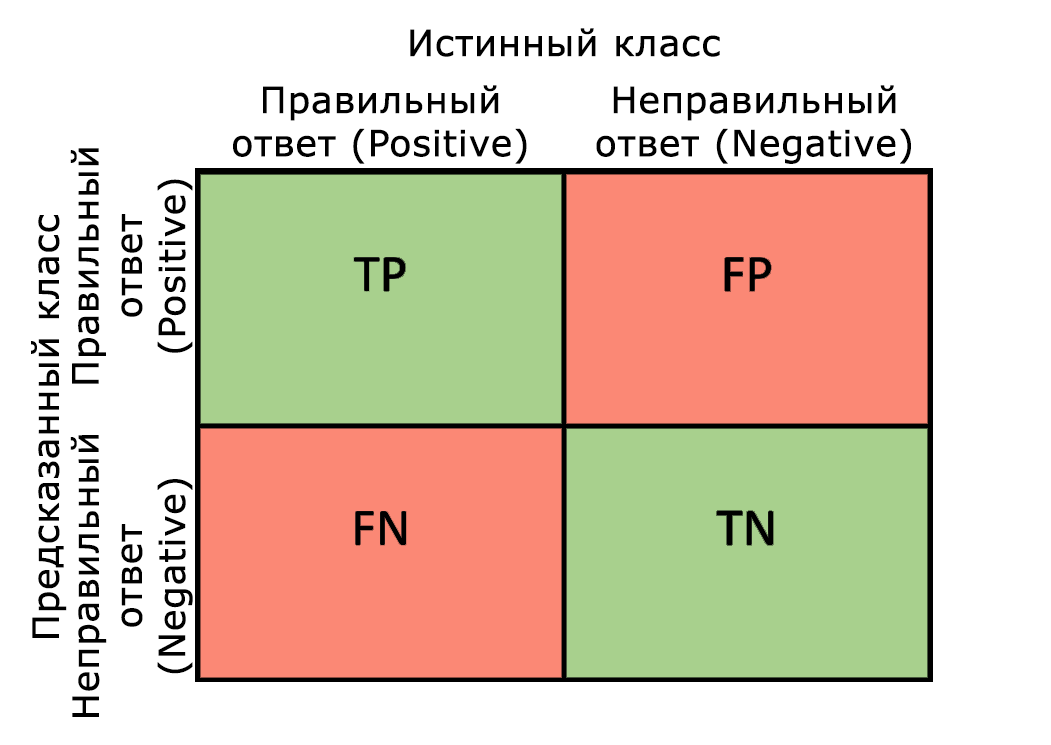
\includegraphics[width=0.6\textwidth]{pics/confusion-matrix.png}
            \caption{Матрица неточностей}
        \end{figure}

        Каждый столбец в этой матрице означает предсказанные экземпляры, в то
        время как каждая строка представляет фактические экземпляры. Таким
        образом, можно сформировать список наиболее известных метрик для
        моделей, решаемых задачу классификации объектов \cite{metrics2}:
        
        \begin{enumerate}
            \item
                Полнота (англ. Recall, а также True Positive Rate или TPR) "---
                это доля найденных классификатором сущностей, принадлежащих
                конкретному классу, относительно всех сущностей этого класса в
                выборке.
                \[TPR = \frac{TP}{TP + FN}\]
            \item
                Точность (англ. Precision, а также Positive Predictive Value
                или PPV) "--- это доля объектов, действительно принадлежащих
                данному классу относительно всех объектов, которые модель
                отнесла к этому классу.
                \[PPV = \frac{TP}{TP + FP}\]
            \item
                Accuracy (ACC) "--- представляет отношение количества верных
                предсказаний к общему количеству образцов выборки.
                \[ACC = \frac{TP + TN}{TP + FP + TN + FN}\]
        \end{enumerate}

        Показатели производительности (англ. performance metrics) или же меры
        ошибки являются необходимыми компонентами в различных сферах применения
        машинного и глубокого обучения. Существует ряд исследований,
        направленных на анализ и классификацию метрик качества обучения модели.
        Наиболее важной для данной работы метрикой оценки модели является та,
        которая позволит оценить качество созданного текстового описания к
        входному изображению, сравнив полученное от нейросети описание с
        истинным, фактическим описанием, созданным человеком для конкретного
        изображения. Для того чтобы сравнивать две последовательности символов
        посредством некоторой метрики, необходимо предварительно каждому из
        символов сопоставить некоторое число, таким образом закодировав текста
        согласно некоторым правилам, после чего осуществить сравнение двух
        векторов, отождествленных с этими описаниями.
    
        Коэффициент Отиаи или же косинусный коэффициент (англ. Cosine \\
        similarity) осуществляет сравнение векторов, определяясь как косинус
        угла $\theta$ между этими двумя векторами $\textbf{y}$ и $\textbf{y'}$:
        
        \[sim(\textbf{y}, \textbf{y'}) = sim_{Cosine}(\textbf{y}, \textbf{y'}) =
        \frac{\langle \textbf{y}, \textbf{y'} \rangle}{\parallel \textbf{y}
        \parallel_2 \cdot \parallel \textbf{y'} \parallel_2 } = \frac{\sum_i y_i
        y'_i}{\sqrt{\sum_i y^2_i} \cdot \sqrt{\sum_i y'^2_i}} = cos \theta \]

        Косинусный коэффициент имеет интересные особенности, которые делают его
        популярным приложением в различных задачах, среди которых наиболее часто
        встречается анализ текста. В первую очередь, легко заметить, что $sim(x,
        y) = sim(\alpha x, y) = sim(x, \alpha y)$ для всех $\alpha > 0$, то есть
        выражение косинусного коэффициента инвариантно к масштабированию
        векторов с положительной скалярной величиной. В случае текстового
        анализа, это является наиболее часто востребованным свойством в силу
        того, что повторяемость содержимого документа несколько раз не меняет
        сущность информации этого текста \cite{metrics3}.     

    \subsection{Функции потерь}

        % CrossEntropyLoss

        В математической оптимизации и теории принятия решений функция потерь
        или функция стоимости (иногда также называемая функцией ошибки) "--- это
        функция, которая отображает событие или значения одной или нескольких
        переменных в действительное число, интуитивно представляющее некоторую
        ''стоимость'', связанную с событием, или же ''погрешность относительно
        эталонного результата''. Задача оптимизации (ровно как и общий смысл
        обучения любой нейросети, модели машинного или глубокого обучения)
        направлена на минимизацию функции потерь. Искомая функция "--- это либо
        функция потерь, либо ее противоположность (в определенных областях она
        по-разному называется функцией вознаграждения, функцией прибыли,
        функцией полезности, функцией пригодности и т. д.), и в этом случае она
        должна быть максимизирована. В статистике обычно функция потерь
        используется для оценки параметров, а рассматриваемое в задаче событие
        является некоторой функцией разницы между оценочными и истинными
        значениями для экземпляра данных \cite{celoss1}.

        % принцип работы функции потерь

        Алгоритмы глубокого обучения используют стохастический градиентный спуск
        для минимизации значения функции потерь и для того, чтобы сгенерировать
        значение целевого признака в качестве ответа. Чтобы узнать ответ точно и
        быстрее, нужно убедиться, что математическое представление ответа, также
        известное как функции потерь, способно охватить даже крайние случаи.
        Введение функций потерь уходит корнями в традиционное машинное обучение,
        где эти функции потерь были получены на основе распределения меток.
        Например, бинарная перекрестная энтропия получена из распределения
        Бернулли, а категориальная перекрестная энтропия - из категориального
        распределения.

        Перекрестная энтропийная потеря (англ. Cross-Entropy Loss) "--- одна из
        наиболее часто используемых функций потерь для обучения глубоких
        нейронных сетей, применение которой особенно популярно при решении задач
        небинарной классификации (то есть типа задачи, в которой в качестве
        результата необходимо получить вектор классов "--- предсказанных
        значений). Работая с категориальными данными, эта функция потерь
        соответствует вероятностному логарифмическому правдоподобию, что
        приводит к благоприятным свойствам оценки. С другой стороны, несколько
        известных методов современного машинного обучения занимаются подгонкой
        данных, которые не столько категориальны, сколько симплекснозначны "---
        например, в такой технике регуляризации обучения, как сглаживание меток
        (англ. Label smoothing), и в работе с определением стратегии агента для
        достижения целей в обучении с подкреплением. В этих методах сообщество
        глубокого обучения по умолчанию заимствовало ту же кросс-энтропийную
        функцию потерь из задачи с категориальными данными, несмотря на то, что
        он больше не определяет целесообразную вероятностную модель
        \cite{celoss2}.

    \subsection{Функции активации}

        % ReLU
        В искусственных нейронных сетях каждый нейрон для своих входных данных
        формирует преобразованную согласно весам этого нейрона сумму и передает
        результирующее скалярное значение через функцию, упоминаемую как функцию
        активации или функцию преобразования. То есть, если нейрон имеет $n$
        входных значений вида $x_1, x_2, \ldots, x_n$, то выходные значения или
        активация нейрона будут выглядеть как $a = g(w_1 \cdot x_1, w_2 \cdot
        x_2, \ldots, w_n \cdot x_n + b)$. Функция $g$ в данном примере является
        функцией активации.
        
        Если в качестве функции $g$ взять линейную функцию $g(z) = z$, тогда
        можно сказать, что нейрон выполняет задачу линейной регрессии или
        классификации. В общем случае $g$ определяется как нелинейная функция
        для решения нелинейной регрессии и задач классификации, которые линейно
        неразделимы. Если функцией активации является сигмоида или $s$-образная
        функция в значениях от $0$ до $1$ или от $-1$ до $1$, результат нейрона
        может быть интерпретирован как 'да' или 'нет' (или в виде выбора между
        двумя значениями).
        
        Стоит отметить, что одной из популярных проблем, связанных с функциями
        активации, является проблема ''насыщения''. Суть её определяется
        состоянием, в котором нейрон преимущественно выдает в качестве
        результата значения, близкие к асимптотическим границам функции
        активации, и это может послужить причиной появления проблемы исчезающего
        градиента в глубоких нейросетях. Замена насыщенных сигмоидальных функций
        активации такими функциями, как ReLU, которые имеют большие
        производные значения, позволяет глубоким нейросетям быть обученными
        гораздо эффективнее. С тех пор появились немонотонные и осциллирующие
        функции активации, значительно превосходящие ReLU в качестве. В
        частности, осциллирующие улучшают градиентный поток, ускоряя обучение и
        позволяя одиночным нейронам учить $XOR$-функцию аналогично некоторым
        человеческим мозговым нейронам \cite{relu2}.

        Функция активации ''выпрямленная линейная единица'', часто называемая
        просто ReLU (сокращение от Rectified Linear Units) имеет сильную
        биологическую и математическую подоплёку. В 2011 году эта функция была
        представлена как дальнейшее улучшение качества обучения глубоких
        нейронных сетей. Она работает с пороговыми значениями в нуле, т.е. $f(x)
        = max(0, x)$. Проще говоря, он выводит $0$, когда $x < 0$, и наоборот,
        он выводит линейную функцию, когда $x \geq 0$ (см. рисунок ниже).

        ReLU менее требовательно к вычислительным ресурсам, чем гиперболический
        тангенс или сигмоида, так как производит более простые математические
        операции. Поэтому имеет смысл использовать ReLu при создании глубоких
        нейронных сетей \cite{relu1}.

        \begin{figure}[H]
            \centering
            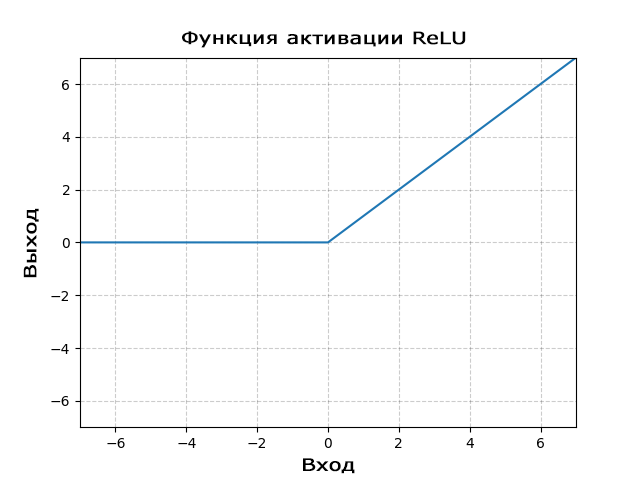
\includegraphics[width=0.8\textwidth]{pics/ReLU.png}
            \caption{Выпрямленная линейная единица (ReLU)}
        \end{figure}

    \subsection{Задачи, решаемые генерацией текстового описания к изображению с помощью нейронной сети}

        Технологии, применяемые для преобразования последовательности пикселей
        изображения в слова с помощью искусственного интеллекта, уже не такие
        безрезультатные, как пять или более лет назад. Более высокая
        производительность, точность и качество делают возможным плавную и
        эффективную генерацию текстового описания к изображениям в различных
        областях — от социальных сетей до электронной коммерции (покупки-продажи
        товаров с помощью цифровых ресурсов). Автоматическое создание тегов,
        соответствующих загруженной фотографии. Эта технология может помочь
        слепым людям познавать окружающий мир.
        
        Как задача взаимодействия визуальных и языковых данных, генерация
        текстового описания к изображениям может быть решена с помощью
        компьютерного зрения и NLP. ИИ подразумевает использование совокупности
        CNN и RNN или любой другой подходящей модели для достижения цели.

        Ниже будут рассматриваются варианты использования технологии генерации
        текстового описания к изображениям \cite{applications}:

        \begin{enumerate}
            \item 
                Расстановка тегов для изображения в рамках электронной
                коммерции, служб обмена фото и онлайн-каталогов. Автоматическое
                создание тегов для фото может упростить жизнь пользователям,
                когда они загружают изображение в онлайн-каталог. В этом случае
                ИИ распознает изображение и генерирует атрибуты "--- это могут
                быть подписи, категории товара или описания. Технология также
                может определять тип товара, материал, цвет, узор и посадку
                одежды для интернет-магазинов. В то же время текстовые описания
                изображений могут быть реализованы службой обмена фотографиями
                или любым онлайн-каталогом для создания автоматического
                осмысленного описания изображения в целях SEO или категоризации.
                Кроме того, подписи позволяют проверить, соответствует ли
                изображение правилам платформы, на которой оно опубликовано.
                Здесь они служат альтернативой категоризации с помощью CNN и
                помогают увеличить трафик и доход.
            \item
                Автоматические аннотации изображений для слепых людей. Чтобы
                разработать такое решение, необходимо преобразовать картинку в
                текст, а затем в голос. Это два хорошо известных применения
                технологии глубокого обучения. Приложение под названием Seeing
                AI, разработанное Microsoft, позволяет людям с проблемами зрения
                видеть окружающий мир с помощью смартфонов. Программа умеет
                читать текст при наведении на него камеры и выдает звуковые
                подсказки. Он может распознавать как печатный, так и рукописный
                текст, а также идентифицировать предметы и людей. Google также
                представил инструмент, который может создавать текстовое
                описание изображения, позволяя слепым или людям с проблемами
                зрения понять контекст изображения или графики. Этот инструмент
                машинного обучения состоит из нескольких слоев. Первая модель
                распознает текст и рукописные цифры на изображении. Затем другая
                модель распознает простые объекты окружающего мира "--- машины,
                деревья, животных и т. д. И третий слой "--- это продвинутая
                модель, способная улавливать основную мысль в полноценном
                текстовом описании.
            \item
                Подписи изображений искусственным интеллектом для социальных
                сетей. Подпись к изображению, созданная с помощью инструмента на
                основе ИИ, уже доступна для Facebook и Instagram. Кроме того,
                модель все время умнеет, учится распознавать новые объекты,
                действия и закономерности. Facebook создал систему, способную
                создавать альтернативные текстовые описания почти пять лет
                назад. В настоящее время она стал более точным. Раньше она
                описывала изображение, используя общие слова, но теперь эта
                система может генерировать подробное описание.
        \end{enumerate}

        \begin{figure}[H]
            \centering
            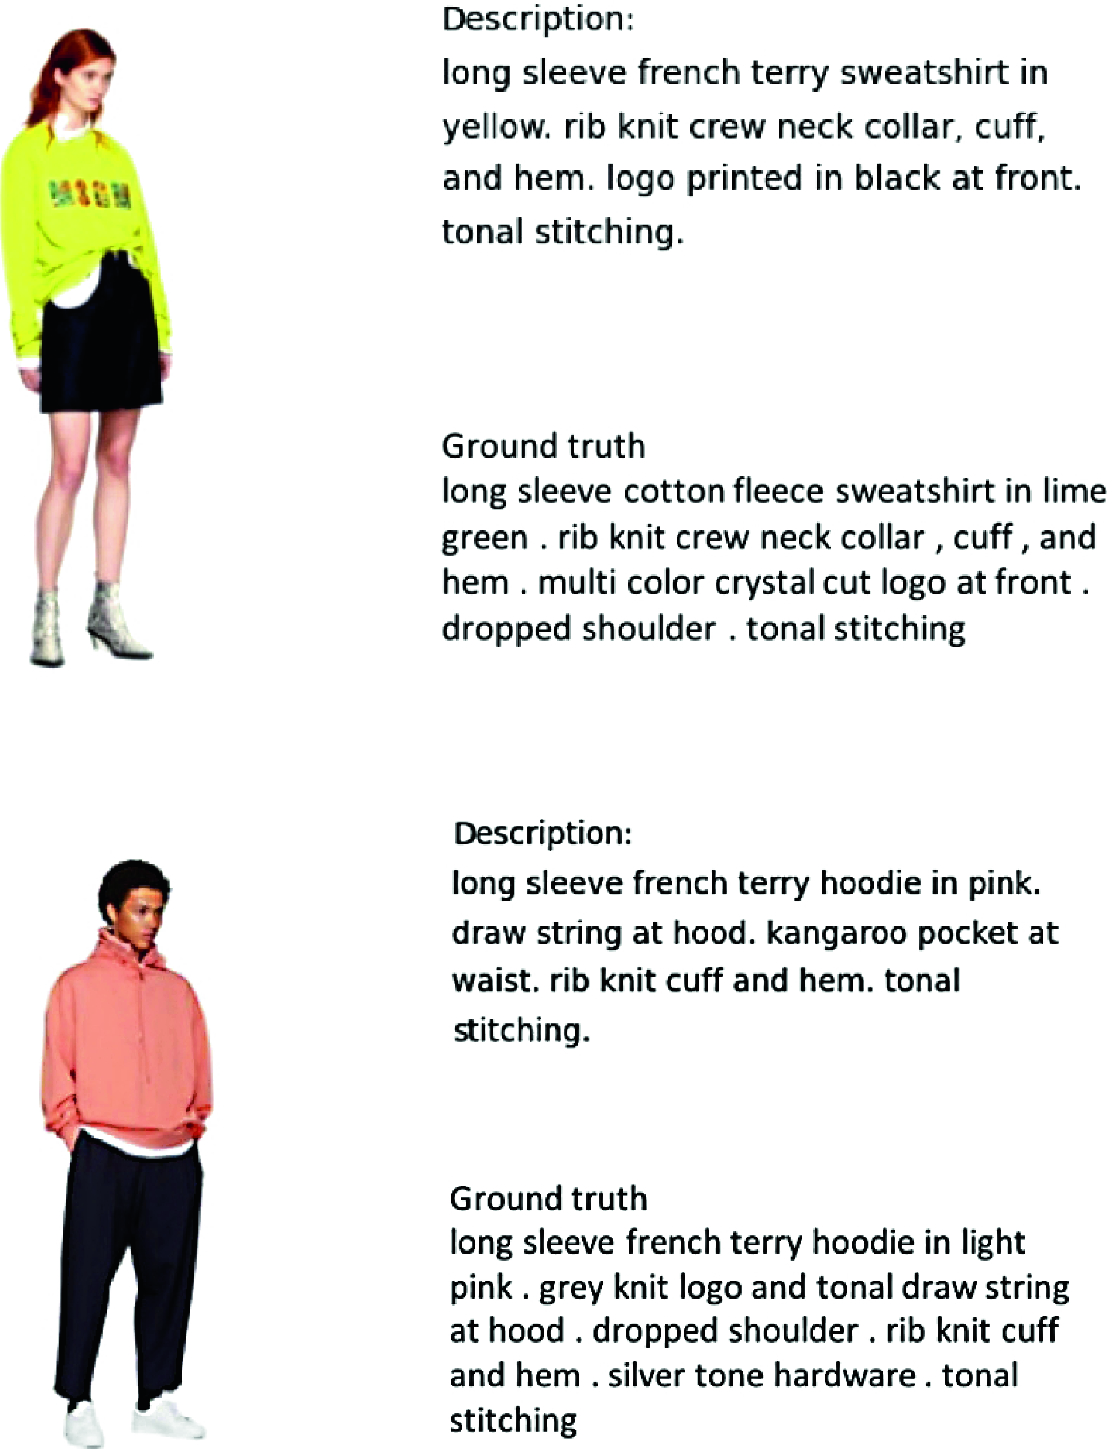
\includegraphics[width=0.8\textwidth]{pics/example.png}
            \caption{Пример применения модели генерации текстового описания для
                     изображения "--- создание описания стиля одежды для
                     магазина}
        \end{figure}

\section{Практическая часть}

    \subsection{Описание инструментов и библиотек программной реализации}

        % Python
        За последние несколько лет Python стал де-факто наиболее привлекательным
        языком для создания, обучения и работы с моделями глубокого обучения
        посредством таких инструментов (англ. framework), как PyTorch,
        TensorFlow, MxNet/TVM и JAX, которые в основном предоставляют интерфейсы
        Python. Простота применения Python для написания кода и возможность его
        распространения через такие пакетные менеджеры, как conda, упрощают
        обмен библиотеками и результатами исследований. Его экосистема библиотек
        для науки о данных, таких как NumPy, Pandas и Jupyter Notebook, упрощают
        анализ результатов обучения моделей и анализ нейросети и данных в целом
        \cite{python}.

        % PIL
        Поскольку программная реализация напрямую подразумевает работу с
        изображениями, для экономии времени и гарантии качества обработки
        входных фото был поднят вопрос касательно выбора инструмента,
        позволяющего осуществлять интерпретацию и ту или иную пред- и
        постобработку картинки. В силу использования Python как основного языка
        для написания кода программной реализации, задача нахождения набора
        инструментов была сведена к поиску подходящей библиотеки для работы с
        изображениями. Для данной задачи и удовлетворения необходимых
        потребностей была выбрана библиотека PIL (сокращение от Python Imaging
        Library). PIL добавляет возможность обработки изображений в
        интерпретатор Python. Эта библиотека обеспечивает обширную поддержку
        форматов файлов, эффективное внутреннее представление и довольно мощные
        возможности процессинга изображений. Основная библиотека изображений
        предназначена для быстрого доступа к данным, хранящимся в нескольких
        основных форматах пикселей. Это должно обеспечить прочную основу для
        общего инструмента обработки изображений \cite{pil}.

        % Pandas
        Так как каждому изображению в обучающей и тестовой выборке должно
        соответствовать как минимум одно текстовое описание, вопрос способа
        сопоставления текста и фото решается с помощью представления этой связи
        в виде таблицы, в которой в первой колонке указывается название фото или
        ссылка на путь к изображению, а во второй колонке записывается текстовое
        описание этой картинки (что является целевым признаком/переменной).
        Способ хранения таких данных непринципиален и основным требованием к
        нему является простота способа взятия данных, поэтому в качестве формата
        хранения таблицы был выбран CSV (сокращение от Comma-Separated Values)
        "--- текстовый формат, предназначенный для представления табличных
        данных. Строка таблицы соответствует строке текста, которая содержит
        одно или несколько полей, разделенных запятыми. Наиболее популярным и в
        то же время самым эффективным способом работы с такого рода
        представлениями данных на языке Python является инструментарий
        библиотеки Pandas. Библиотека Pandas предоставляет структуры данных и
        функции, призванные сделать работу со структурированными данными
        простой, быстрой и выразительной. С момента появления в 2010 году она
        способствовала превращению Python в мощную и продуктивную среду анализа
        данных. Основные объекты Pandas "--- это DataFrame "--- двумерная
        таблица, в  которой строки и столбцы имеют метки, и Series "--- объект
        одномерного массива с  метками. В библиотеке Pandas сочетаются высокая
        производительность средств работы с массивами, присущая NumPy, и гибкие
        возможности манипулирования данными, свойственные электронным таблицам и
        реляционным базам данных (например, на основе SQL). Она предоставляет
        развитые средства индексирования, позволяющие без труда изменять форму
        наборов данных, формировать продольные и  поперечные срезы, выполнять
        агрегирование и выбирать подмножества \cite{pandas}.
        
        % Spacy
        Помимо обработки изображений и табличных данных, необходимо осуществлять
        корректную обработку самих текстов, подготовленных для обучения и
        тестирования модели, и контролировать генерацию текстовых описаний
        посредством сильного инструмента. SpaCy обеспечивает надежную
        архитектуру для создания и совместного использования пользовательских
        высокопроизводительных конвейеров NLP (англ. pipeline), принимая
        объектно-ориентированное представление текста. Он не деструктивен,
        поддерживает плавную интеграцию статистических методов и методов
        машинного обучения с NLP, построенном на основе правил, и позволяет
        создавать пользовательские компоненты для специализированных задач.
        Благодаря возможностям Cython, оптимизирующего статического компилятора
        для Python, который генерирует очень эффективный код C или C++, spaCy
        позволяет достичь исключительной скорости работы. Подобно подходу UIMA в
        Java, spaCy предоставляет основу для модульного построения настраиваемых
        конвейеров NLP по принципу plug-and-play. С момента своего создания в
        2015 году, библиотека spaCy приобрела сильное, очень активное и растущее
        сообщество разработчиков модулей с открытым исходным кодом, современными
        моделями и комплексными системами, разработанными с помощью платформы
        или для неё самой \cite{spacy}.
        
        % PyTorch
        Фреймворки глубокого обучения часто фокусируются либо на удобстве своего
        использования, либо на скорости работы. PyTorch "--- это библиотека
        машинного обучения, которая показывает, что эти две цели на самом деле
        совместимы: она обеспечивает императивный и Python-подобный стиль
        программирования, который поддерживает код как модель, упрощает отладку
        и согласуется с другими научно-популярными вычислительными библиотеками,
        оставаясь при этом эффективным и поддерживая аппаратные ускорители,
        такие как графические процессоры. Популярность PyTorch связана с
        объединением технических идей реализации библиотеки с дизайном, который
        сочетает в себе баланс скорости и лёгкости использования. В основе
        дизайна лежат четыре основных принципа \cite{pytorch}:

        \begin{enumerate}
            \item
                Быть Python-подобным. Подавляющее большинство специалистов по
                анализу данных знакомо с языком Python, его подходами к
                программированию и инструментами. PyTorch должен быть
                первоклассным членом этой экосистемы. Это ведет к общепринятым
                идеям дизайна "--- сделать интерфейс взаимодействия простым и
                согласованным, в идеале с одним идиоматическим способом создания
                решений задач машинного обучения. Он также естественным образом
                интегрируется со стандартными инструментами построения графиков,
                отладки и обработки данных.
            \item
                Первостепенная важность исследователей. PyTorch стремится
                сделать написание моделей, загрузчиков данных и оптимизаторов
                как можно легче и продуктивнее. Сложность, присущая машинному
                обучению, должна быть решена внутренне библиотекой PyTorch и
                скрыта за интуитивно понятным API без побочных эффектов и
                неожиданных нюансов в производительности.
            \item
                Обеспечение прагматичной производительности. Чтобы быть
                полезным, PyTorch должен обеспечивать существенную
                производительность, хотя и в небольшой ущерб простоте и удобству
                использования. Обменять 10\% скорости на значительно упрощенную
                реализацию использования модели вполне приемлемо, но терять
                100\% быстродействия для этого "--- недопустимо. Поэтому
                библиотека допускает добавление сложности для обеспечения этой
                производительности. Кроме того, предоставление инструментов,
                позволяющих исследователям вручную управлять выполнением своего
                кода, позволит им найти собственную планку производительности,
                независимую от тех, которые библиотека предоставляет
                автоматически.
            \item
                Чем хуже, тем лучше. При фиксированном количестве инженерных
                ресурсов и прочих равных условиях, время, сэкономленное за счет
                упрощения внутренней реализации PyTorch, можно использовать для
                реализации дополнительных функций, адаптирования к новым
                ситуациям, таким образом идя в ногу с быстрыми темпами прогресса
                в области ИИ. Поэтому лучше иметь простое, но немного неполное
                решение, чем всеобъемлющую, но сложную и неудобную в
                обслуживании конструкцию.
        \end{enumerate}
        
    \subsection{Описание набора данных для обучения и теста}

        Осуществление предобработки и принятие решения о выборе того или иного
        набора данных для конкретной задачи машинного или глубокого обучения
        является столь же важным этапом деятельности создания ИИ, как и
        проектирование архитектуры модели и сопровождение процесса обучения.

        В данной работе осуществляется решение задачи генерации текстового
        описания к изображению "--- следовательно, рациональнее и эффективнее
        следует взять в качестве основного ресурса для обучения нейросети один
        из таких наборов данных, как ''Microsoft COCO'', ''Visual Genome'',
        ''TextCaps'', ''Flickr 8k'' и т.п. В качестве основополагающих данных
        необязательно брать большой объем изображений с их текстовым описанием
        "--- для проверки качества реализации нейросети достаточно выбрать
        умеренное количество информации, и в связи с этим было принято решение
        выбрать набор данных ''Flickr 8k'' (то есть исходя из других различных
        исследовательских работ, связанных с генерацией текстового описания к
        изображению) \cite{dataset1}, \cite{dataset2}.
        
        Набор представляет собой эталонную коллекцию для генерации текстового
        описания и поиска изображений на основе предложений на естественном
        языке, которая состоит из более чем 8000 изображений, каждое из которых
        имеет пять разных текстовых подписей, которые обеспечивают четкое
        описание фигурирующих на конкретном изображении объектов и событий.
        Изображения были выбраны из шести разных групп Flickr и, как правило, не
        содержат каких-либо известных людей или мест, а были отобраны вручную
        для отображения различных мероприятий и ситуаций. Набор данных находится
        в открытом доступе и его можно загрузить как с официального сайта
        фотохостинга, так и с других различных форумов и сайтов для машинного и
        глубокого обучения \cite{dataset3}. В частности, для обучения модели,
        описывающейся в данной работе, была взята такая коллекция совместно с
        файлом формата CSV, в котором осуществляется сопоставление названия
        каждого изображения с одним из его текстовых описаний.

        Эти данные будут в дальнейшем поделены на тренировочную и тестовую
        выборку, где первая выборка будет представлять собой 80\% от всего
        набора данных, а тестовая "--- всё остальное.

        \begin{figure}[H]
            \centering
            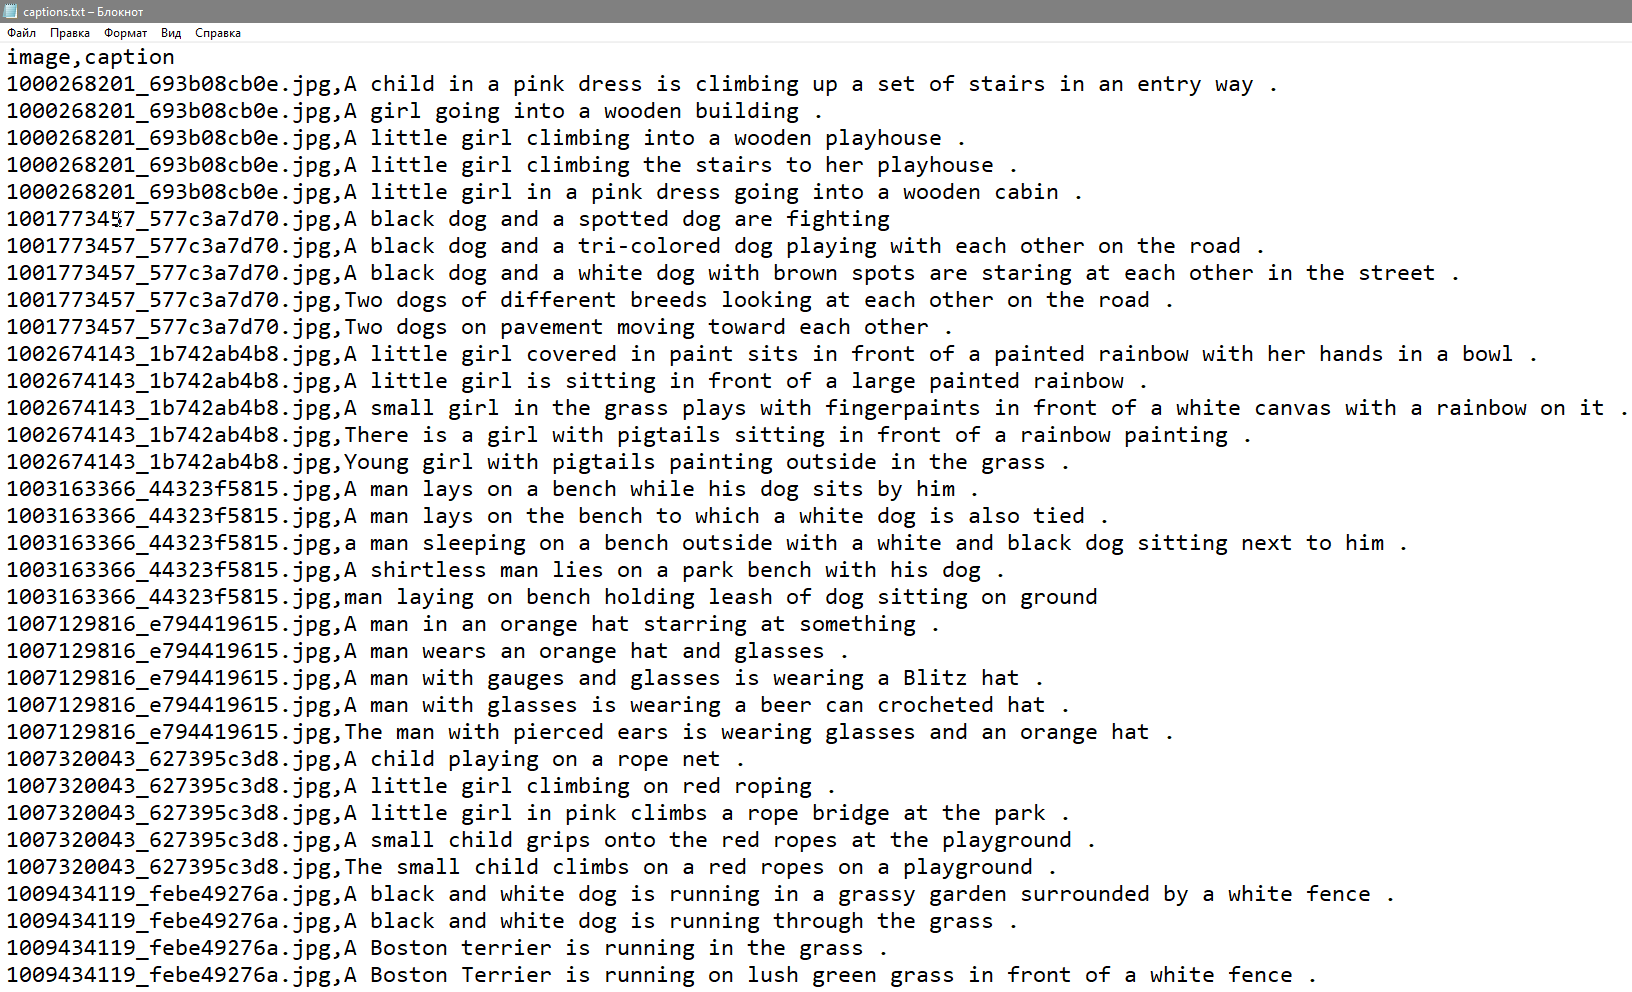
\includegraphics[width=1\textwidth]{pics/dataset.png}
            \caption{Содержимое CSV файла, в котором сопоставляется изображение
                     с текстовым описанием}
        \end{figure}


    \subsection{Программная реализация алгоритма}

        Генератор подписей к входным изображениям будет представлять собой
        ансамбль из двух нейросетей - CNN и LSTM.

        Идея работы ансамбля заключается в том, что на вход к CNN подается
        цветное изображение (размеры которого предварительно сведены к 356
        пикселя в ширину и 356 пикселя в высоту). В качестве CNN будет
        использоваться модель GoogleNetv3, предобученная на датасете 2015-го
        года ImageNet.
        
        Предобученная модель основана на исследовании способов масштабирования
        сетей таким образом, чтобы максимально эффективно использовать
        дополнительные вычисления за счет подходящей факторизованной свертки и
        агрессивной регуляризации. В официальной документации библиотеки PyTorch
        можно посмотреть статистику работы данной нейросети с набором тестовых
        задач классификации ILSVRC 2012, которые демонстрируют хорошее качество
        модели \cite{inception}.
        
        Получая на вход изображение в виде тензора, она будет пропускать его
        через все свои слои, и из последнего полностью соединенного слоя
        нейросети будет выдавать некоторый вектор, который впоследствии
        преобразуется с помощью линейного слоя. Таким образом, CNN в данной
        архитектуре будет являться своего рода кодировщиком, выдавая для каждого
        конкретного изображения некоторый вектор.
        
        Полученный обработанный вектор отправляется на вход нейросети LSTM,
        которая (с учетом определенного словаря, количества lstm-слоев и прочих
        гиперпараметров) будет создавать последовательные связанные друг с
        другом слова. 
        
        LSTM-модель обучена предсказывать каждое слово предложения после
        получения входного изображения таким же образом как и предшествующие
        слова (это можно определить как $P(S_t | I, S_0, S_1, ..., S_{t - 1})$).
        Для этого следует определить работу LSTM в развернутом виде. Копия
        памяти LSTM для изображения, а также каждое слово предложения (такое,
        которое определяет для всех LSTM-модулей одни и те же параметры) и выход
        $m_{t - 1}$ модуля LSTM в момент времени $t - 1$ подаются на вход к
        модулю LSTM в момент времени $t$. В развернутом виде все рекуррентные
        соединения преобразуются в соединения прямой связи. Если рассматривать
        более детально, то если определить $I$ как входное изображение, для
        которого задано исходное текстовое описание в виде $S = S_0, ..., S_N$,
        то процедура развертывания выглядит следующим образом:
        
        % The LSTM model is trained to predict each word of the sentence after it
        % has seen the image as well as all preceding words as defined by $P(S_t |
        % I, S_0, S_1, ..., S_{t - 1})$. For this purpose, it is instructive to
        % think of the LSTM in unrolled form; a copy of the LSTM memory is created
        % for the image and each sentence word such that all LSTMs share the same
        % parameters and the output $m_t - 1$ of the LSTM at time $t - 1$ is fed
        % to the LSTM at time $t$. All recurrent connections are transformed to
        % feedforward connections in the unrolled version. In more detail, if we
        % denote by $I$ the input image and by $S = S_0, ..., S_N$ a true sentence
        % describing this image, the unrolling procedure reads

        \[X_{-1} = CNN(I) \]
        \[x_t = W_e S_t, t \in \{0...N - 1 \} \]
        \[p_{t + 1} = LSTM(x_t), t \in \{0...N - 1 \} \]

        где каждое слово представляется унитарно закодированным вектором (англ.
        one-hot vector) размерности, равной размеру словаря. Следует отметить,
        что в качестве $S_0$ задается токен, определяющий начало предложения, а
        в качестве $S_N$ "--- токен, определяющий конец предложения. В
        частности, с помощью токена конца предложения LSTM сигнализирует о том,
        что текстовое описание было полностью сгенерировано. И изображение, и
        слова сопоставляются к одному пространству: изображение с помощью CNN,
        слова с помощью эмбэддинга слов $W_e$. Изображение $I$ подается на вход
        только один раз, в момент времени $t = -1$, чтобы передать информацию
        модулю LSTM о своём содержании \cite{dataset1}.

        Это делает LSTM-модель своего рода декодировщиком, результатом
        деятельности которого будет подпись к изображению.

        \begin{figure}[H]
            \centering
            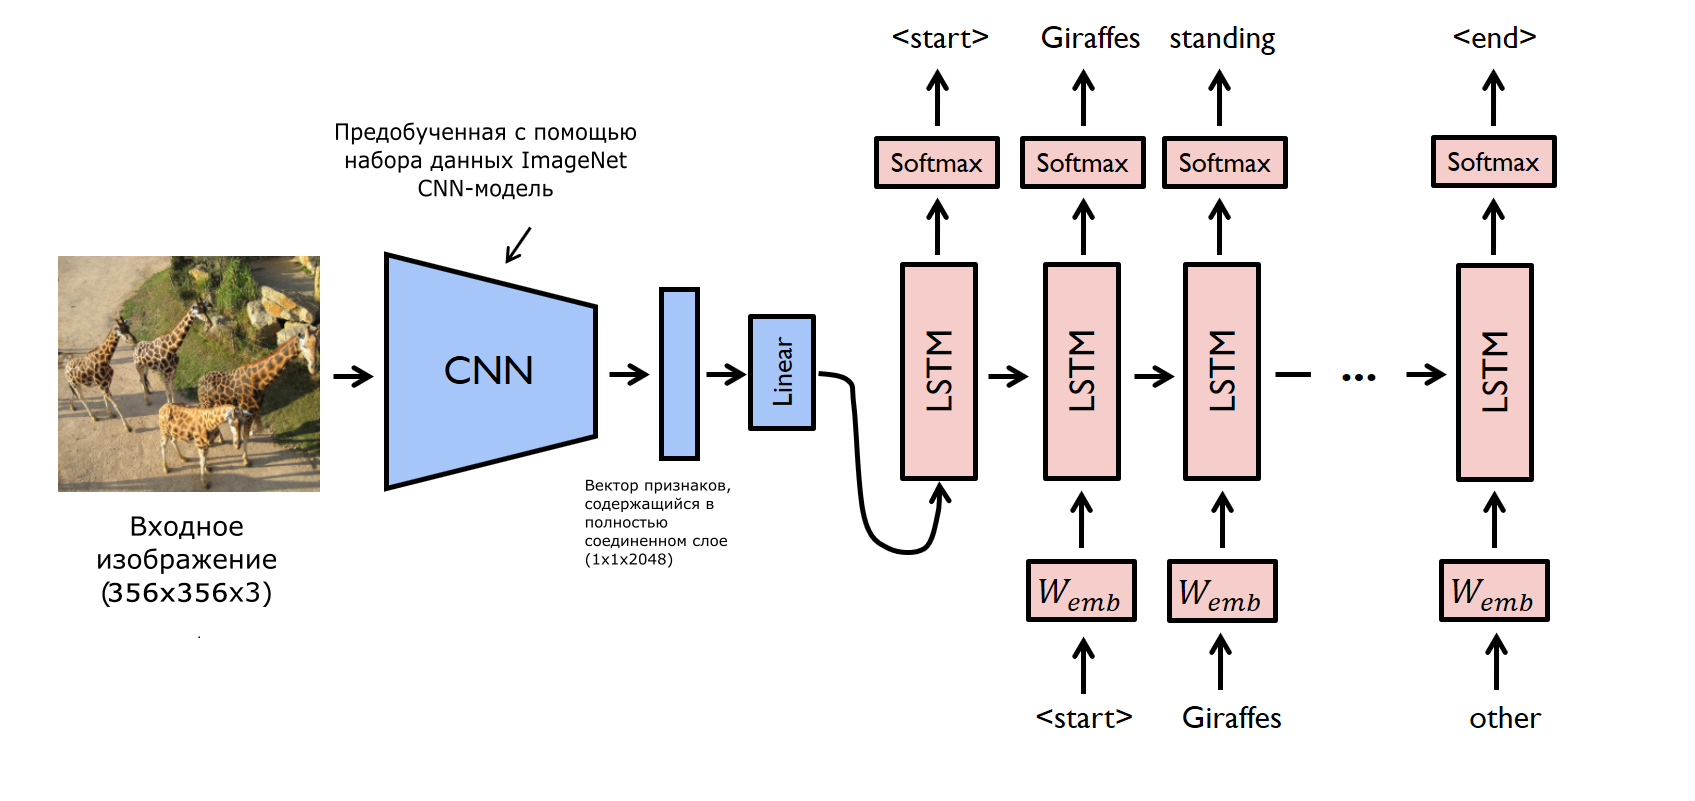
\includegraphics[width=1\textwidth]{pics/arch.png}
            \caption{Архитектура программы}
        \end{figure}

    \subsection{Приведение характеристик обучения и гиперпараметров}

        В большинстве случаев применения, размер эмбэддинга (англ. embedding
        size) определяется эмпирическим путем, через ошибки и в процессе
        улучшения качества обучения модели. Старые работы на тему NLP
        использовали значение 300. Более свежие работы используют размер, равный
        512, 768 и 1024. Одним из факторов, влияющих на выбор размера является
        то, каким образом предпочтительнее осуществлять корреляцию различных
        векторов друг с другом. В пространстве высокой размерности с
        вероятностью 1, выбранные случайным образом векторы будут приблизительно
        взаимно ортогональны. В то время как при малых размерностях и в случае
        множества различных классов, многие векторы будут иметь скалярное
        произведение, значение которого значительно отличается от нуля. Если
        ожидать, что многие векторы должны быть коррелированными, размерность не
        должна быть очень высокой. В противном случае, если ожидается, что
        каждый из возможных ключей эмбэддинга будет создавать другой,
        несвязанный вектор, тогда размерность следует выбрать большой. В
        качестве изначального значения размера эмбэддинга было выбрано число
        256, аналогично количеству выходных векторов LSTM \cite{embedding}.
        
        Размер словаря, с помощью которого будет формироваться текстовое
        описание для каждого изображения, определяется напрямую количеством
        уникальных слов, найденных в CSV-файле набора данных, а также NLP
        токенами типа ''начало предложения'', ''конец предложения'' и т.д.
        
        Начальное количество слоев LSTM (то есть количество идущих подряд
        модулей LSTM) задано числом 2, и при необходимости может установиться с
        иным значением.
        
        Говоря о темпе обучения (англ. learning rate), разработчики Tensorflow,
        Pytorch и другие в своей документации рекомендуют установить значение
        темпа обучения равным 0.001. Однако в решении университета Станфорд
        задачи генерации текстового описания начальное значение этого параметра
        для LSTM-сети было выбрано 0.0004, что также послужило основной для
        определения темпа обучения сети-кодировщика в данной работе
        \cite{learningrate}.
        
        Количество эпох обучения определено значением 100.

        % Обучение ансамбля происходило на домашнем компьютере с поддержкой
        % технологии CUDA (в силу наличия видеокарты Nvidia)

    \subsection{Результаты обучения}

        Для того, чтобы проверить качество обучения модели (то есть
        проконтролировать отсутствие переобучения и недообучения, вследствие
        которых модель может работать плохо, согласно оцениваемой метрике), в
        процессе обучения сохранялись значения функции ошибки согласно
        конкретному моменту времени. Используя эти параметры, можно построить
        график зависимости перекрестной энтропийной потери от времени
        (называемой кривой обучения), чтобы проследить, уменьшается ли значение
        ошибки с каждой итерацией или нет.
        
        % график кривой обучения
        \begin{figure}[H]
            \centering
            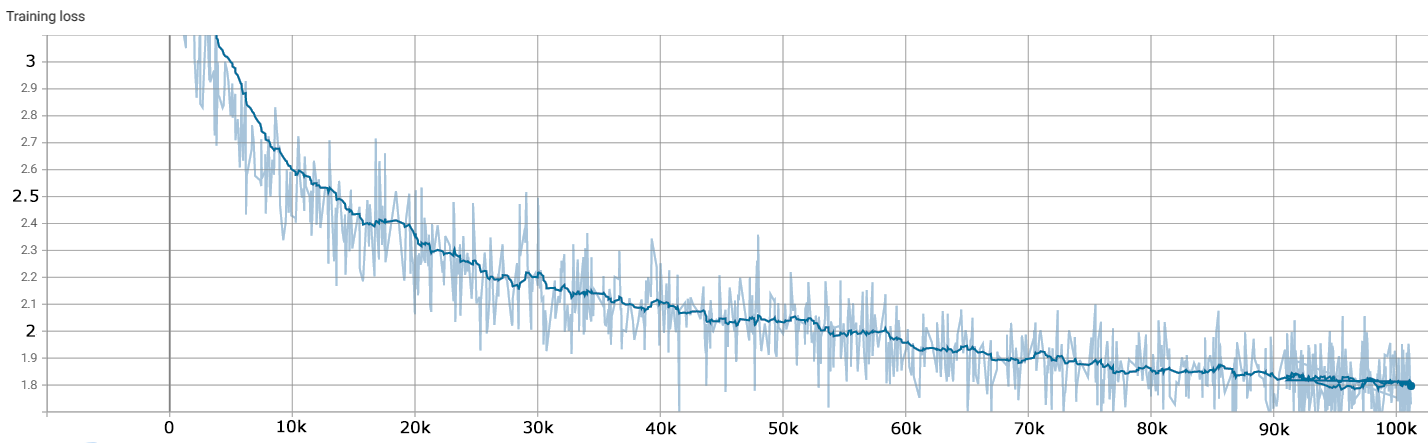
\includegraphics[width=1\textwidth]{pics/curve.png}
            \caption{График кривой обучения, где вдоль оси OY обозначены
                     значения функции потерь, а вдоль оси OX "--- номер
                     итерации}
        \end{figure}

        Согласно изображению выше можно сказать, что процесс обучения проходил
        без каких-либо сложностей, и признаков недообучения и переобучения на
        данном графике не обнаружено \cite{fitting}.

        Для осуществления оценки работы модели с помощью выбранной ранее
        метрики, предварительно следует подчеркнуть создание функции, которая
        получает на вход изображение, и генерирует с помощью созданной нейросети
        текстовое описание на английском языке.

        % пример генерации текстового описания
        \begin{figure}[H]
            \centering
            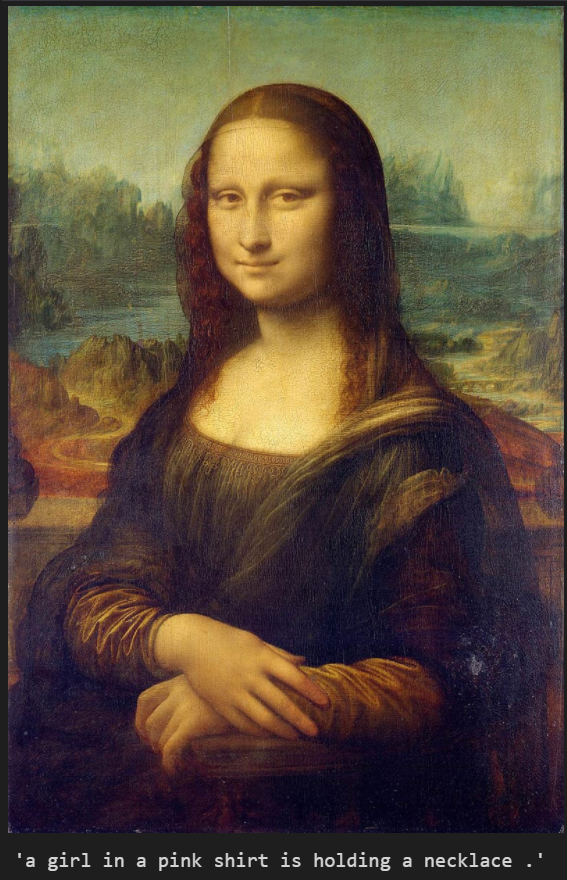
\includegraphics[width=0.6\textwidth]{pics/caption.png}
            \caption{Пример генерации текстового описания}
        \end{figure}

        Используя методы библиотеки NumPy, можно создать метрику, упомянутую
        ранее как косинусный коэффициент, с помощью которой можно осуществить
        проверку качества модели. Для этого была написана функция, которая будет
        получать в качестве аргумента тестовую выборку, и с помощью модели
        генерировать предсказания, которые затем будут использоваться метрикой
        для оценки посредством применения косинусного коэффициента к
        предсказанию и эталонному текстовому описанию. Затем следует взять
        среднее значение от результата работы метрики для всех изображений,
        которое и будет являться средним значением качества данной модели.
        
        Эта средняя оценка будет представлена действительным числом, которое
        находится в диапазоне значений от 0 до 1 (чем ближе значение к 1, тем
        лучше качество). Однако у человека, который не понимает принципов работы
        данной оценки, будут возникать проблемы понимания того, хороша ли модель
        или нет. Поэтому функция выше была дополнена возможностью, которая
        интерпретирует значение оценки в более понятный вид разделением
        диапазона значений на 4 промежутка. Это означает, что:
        
        \begin{enumerate}
            \item Значение метрики от 0 до 0.25 приведет к возврату данной
            функцией строки ''Модель работает плохо, не способна даже в общих
            чертах описать то, что присутствует на изображении.'';
            \item Значение от 0.25 до 0.5 "--- ''Модель работает
            удовлетворительно "--- способна различать и корректно
            интерпретировать основные детали изображения, но может допускать
            некоторые логические и смысловые ошибки в описании.'';
            \item от 0.5 до 0.75 "--- ''Модель работает хорошо "--- почти всегда
            корректно описывает основные детали изображения, но способна
            допускать незначительные логические ошибки.'';
            \item от 0.75 "--- ''Модель работает отлично, количество ошибок при
            генерации текстового описания к входному изображению сведено к
            минимуму.''
        \end{enumerate}

        % пример вывода действительного и интерпретированного значения метрики
        \begin{figure}[H]
            \centering
            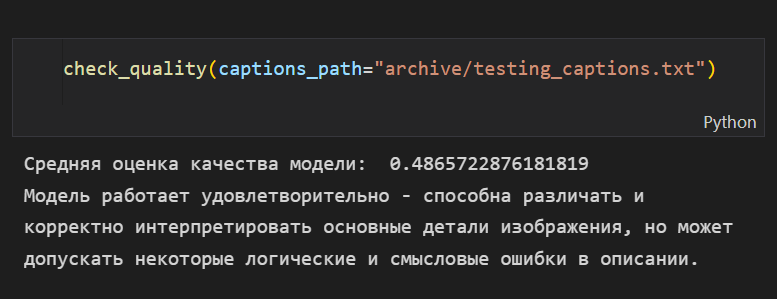
\includegraphics[width=1\textwidth]{pics/metriceval.png}
            \caption{Вывод действительного и интерпретированного
                     значения метрики}
        \end{figure}

\conclusion

    В данной работе был рассмотрен метод решения задачи генерации текстового
    описания к изображению путём построения ансамбля из двух видов нейросетей. В
    связи с этим, предварительно были рассмотрены теоретические понятия
    искусственных, сверточных, рекуррентных нейросетей, описаны основные
    принципы работы этих видов сетей и их роль в решении. Также были приведены
    описания таких терминов, как функции потерь, функции активации, метрики
    оценки качества обучения, перечислены их виды (в том числе описаны те, что
    применяются конкретно в этой задаче) и указана их важная роль в науке о
    машинном и глубоком обучении.
    
    В качестве практической части работы была описана программная реализация
    алгоритма генерации текстового описания к изображению и рассмотрена
    архитектура ансамбля используемых нейросетей. Согласно обозначенным
    гиперпараметрам, было осуществлено обучение модели, результаты которого
    также были представлены посредством графиков кривой обучения, демонстрации
    генерации текстового описания к изображению и вычислению среднего значения
    выбранной метрики. Качество работы ансамбля, оцененное метрикой, можно
    считать средним, но вместе с тем доступным к улучшению с помощью подбора
    гиперпараметров.

\begin{thebibliography}{99}
    \bibitem{neur} Короткий С., ''Нейронные сети: Основные положения'',
    [Электронный ресурс] : [статья] / URL:
    http://www.shestopaloff.ca/kyriako/Russian/Artificial_Intelligence/Some_publications/Korotky_Neuron_network_Lectures.pdf
    (дата обращения 27.04.2022) Загл. с экрана. Яз. рус.
    
    \bibitem{Gud} Гудфеллоу Я., Бенджио И., Курвилль А., ''Глубокое обучение'',
    г. Москва, Издательство ДМК, 2018 г., Яз. рус.
    
    % CNN
    % https://arxiv.org/abs/1511.08458
    % https://www.freecodecamp.org/news/an-intuitive-guide-to-convolutional-neural-networks-260c2de0a050/

    \bibitem{cnn1} Keiron O'Shea, Ryan Nash, ''An Introduction to Convolutional
    Neural Networks'', [Электронный ресурс] : [статья] / URL
    https://arxiv.org/abs/1511.08458 (дата обращения 14.04.2022) Загл. с экрана.
    Яз. англ.
    
    \bibitem{cnn2} Daphne Cornelisse, ''An intuitive guide to Convolutional
    Neural Networks'', [Электронный ресурс] : [статья] / URL
    https://www.freecodecamp.org/news/an-intuitive-guide-to-convolutional-neural-networks-260c2de0a050/
    (дата обращения 14.04.2022) Загл. с экрана. Яз. англ.

    % RNN
    % https://arxiv.org/pdf/1912.05911.pdf
    % https://www.ibm.com/cloud/learn/recurrent-neural-networks
    
    \bibitem{rnn1} Robin M. Schmidt, ''Recurrent Neural Networks (RNNs): A
    gentle Introduction and Overview'', [Электронный ресурс] : [статья] / URL
    https://arxiv.org/pdf/1912.05911.pdf (дата обращения 18.04.2022) Загл. с
    экрана. Яз. англ.

    \bibitem{rnn2} IBM Cloud Education, ''Recurrent Neural Networks'',
    [Электронный ресурс] : [статья] / URL
    https://www.ibm.com/cloud/learn/recurrent-neural-networks (дата обращения
    18.04.2022) Загл. с экрана. Яз. англ.

    % LSTM
    % https://arxiv.org/pdf/1909.09586.pdf
    % https://habr.com/ru/company/wunderfund/blog/331310/

    \bibitem{lstm1} Ralf C. Staudemeyer, Eric Rothstein Morris, ''Understanding
    LSTM "--- a tutorial into Long Short-Term Memory Recurrent Neural Networks
    '', [Электронный ресурс] : [статья] / URL
    https://arxiv.org/pdf/1909.09586.pdf (дата обращения 22.04.2022) Загл. с
    экрана. Яз. англ.

    \bibitem{lstm2} Wunder Fund, ''LSTM – сети долгой краткосрочной памяти'',
    [Электронный ресурс] : [статья] / URL
    https://habr.com/ru/company/wunderfund/blog/331310/ (дата обращения
    22.04.2022) Загл. с экрана. Яз. рус.

    % Metrics
    % https://arxiv.org/ftp/arxiv/papers/1809/1809.03006.pdf
    % https://arxiv.org/ftp/arxiv/papers/2006/2006.00887.pdf
    % https://arxiv.org/pdf/1208.3145.pdf

    \bibitem{metrics1} Alexei Botchkarev, ''Performance Metrics (Error Measures)
    in Machine Learning Regression, Forecasting and Prognostics: Properties and
    Typology'', [Электронный ресурс] : [статья] / URL
    https://arxiv.org/ftp/arxiv/papers/1809/1809.03006.pdf (дата обращения
    24.04.2022) Загл. с экрана. Яз. англ.

    \bibitem{metrics2} M.Z. Naser, Amir H. Alavi, ''Insights into Performance
    Fitness and Error Metrics for Machine Learning'', [Электронный ресурс] :
    [статья] / URL https://arxiv.org/ftp/arxiv/papers/2006/2006.00887.pdf (дата
    обращения 24.04.2022) Загл. с экрана. Яз. англ.

    \bibitem{metrics3} Stijn Van dongen, Anton J. Enright, ''METRIC DISTANCES
    DERIVED FROM COSINE SIMILARITY AND PEARSON AND SPEARMAN CORRELATIONS'',
    [Электронный ресурс] : [статья] / URL https://arxiv.org/pdf/1208.3145.pdf
    (дата обращения 24.04.2022) Загл. с экрана. Яз. англ.

    % Cross Entropy Loss
    % https://arxiv.org/pdf/2011.05231.pdf
    % https://arxiv.org/pdf/2006.14822.pdf

    \bibitem{celoss1} Elliott Gordon-Rodriguez, Gabriel Loaiza-Ganem и т.д.,
    ''Uses and Abuses of the Cross-Entropy Loss: Case Studies in Modern Deep
    Learning'', [Электронный ресурс] : [статья] / URL
    https://arxiv.org/pdf/2011.05231.pdf (дата обращения 27.04.2022) Загл. с
    экрана. Яз. англ.

    \bibitem{celoss2} Shruti Jadon, ''A survey of loss functions for semantic
    segmentation'', [Электронный ресурс] : [статья] / URL
    https://arxiv.org/pdf/2006.14822.pdf (дата обращения 27.04.2022) Загл. с
    экрана. Яз. англ.

    % Relu
    % https://arxiv.org/pdf/1803.08375.pdf
    % https://arxiv.org/pdf/2107.09370.pdf

    \bibitem{relu1} Abien Fred M. Agarap, ''Deep Learning using Rectified Linear
    Units (ReLU)'', [Электронный ресурс] : [статья] / URL
    https://arxiv.org/pdf/1803.08375.pdf (дата обращения 28.04.2022) Загл. с
    экрана. Яз. англ.

    \bibitem{relu2} Pierre Stock, Remi Gribonval, ''AN EMBEDDING OF RELU
    NETWORKS AND AN ANALYSIS OF THEIR IDENTIFIABILITY'', [Электронный ресурс] :
    [статья] / URL https://arxiv.org/pdf/2107.09370.pdf (дата обращения
    28.04.2022) Загл. с экрана. Яз. англ.
    

    % https://mobidev.biz/blog/exploring-deep-learning-image-captioning
    \bibitem{applications} Diana Malyk, ''Exploring Deep Learning Image
    Captioning'', [Электронный ресурс] : [статья] / URL
    https://mobidev.biz/blog/exploring-deep-learning-image-captioning (дата
    обращения 30.04.2022) Загл. с экрана. Яз. англ.

    % Python
    % https://arxiv.org/pdf/2104.00254.pdf
    \bibitem{python} Zachary DeVito, Jason Ansel и т.д., ''USING PYTHON FOR MODEL
    INFERENCE IN DEEP LEARNING'', [Электронный ресурс] : [статья] / URL
    https://arxiv.org/pdf/2104.00254.pdf (дата обращения 2.05.2022) Загл. с
    экрана. Яз. англ.
    % PIL
    % https://pypi.org/project/Pillow/
    \bibitem{pil} Alex Clark и т.д., ''Pillow'', [Электронный ресурс] : [статья]
    / URL https://pillow.readthedocs.io/en/stable/ (дата обращения 2.05.2022)
    Загл. с экрана. Яз. англ.
    % Pandas
    % https://vk.com/doc44301783_570833604?hash=LGYlshZgzLYwudBTZs1qE7XYb8l9puWt8uHniCTh6Zs&dl=icFVk5kLe613AvNLwIwLfFlkaiWT6odCWzRf3ZMgQXL
    \bibitem{pandas} Маккинни У., ''Python и анализ данных'', ДМК Пресс, 2015.
    "--- 482 с. "--- ISBN 978-5-97060-315-4, 978-1-449-31979-3.
    % Spacy
    % https://arxiv.org/pdf/2106.07799.pdf
    \bibitem{spacy} Hannah Eyre, Alec B Chapman и т.д., ''Launching into clinical
    space with medspaCy: a new clinical text processing toolkit in Python'',
    [Электронный ресурс] : [статья] / URL https://arxiv.org/pdf/2106.07799.pdf
    (дата обращения 2.05.2022) Загл. с экрана. Яз. англ.
    % PyTorch
    \bibitem{pytorch} Adam Paszke, Sam Gross и т.д., ''PyTorch: An Imperative
    Style, High-Performance Deep Learning Library'', [Электронный ресурс] :
    [статья] / URL https://arxiv.org/pdf/1912.01703.pdf (дата обращения
    2.05.2022) Загл. с экрана. Яз. англ.
    % Torchvision

    % Dataset
    \bibitem{dataset1} Vikram Mullachery, Vishal Motwani, ''Image Captioning'',
    [Электронный ресурс] : [статья] / URL https://arxiv.org/pdf/1805.09137.pdf
    (дата обращения 8.05.2022) Загл. с экрана. Яз. англ.

    \bibitem{dataset2} Kelvin Xu, Jimmy Lei Ba и т.д., ''Show, Attend and
    Tell: Neural Image Caption Generation with Visual Attention'', [Электронный
    ресурс] : [статья] / URL https://arxiv.org/pdf/1502.03044.pdf (дата
    обращения 8.05.2022) Загл. с экрана. Яз. англ.

    \bibitem{dataset3} ADITYAJN105, ''Flickr 8k Dataset '', [Электронный ресурс]
    : [статья] / URL https://www.kaggle.com/datasets/adityajn105/flickr8k (дата
    обращения 8.05.2022) Загл. с экрана. Яз. англ.

    % model

    \bibitem{inception} Pytorch Team, ''INCEPTION_V3'', [Электронный ресурс] :
    [статья] / URL https://pytorch.org/hub/pytorch_vision_inception_v3/ (дата
    обращения 8.05.2022) Загл. с экрана. Яз. англ.

    % hyperparams

    \bibitem{embedding} Adam Schwab, ''Embeddings: A Matrix of Meaning'',
    [Электронный ресурс] : [статья] / URL
    https://petuum.medium.com/embeddings-a-matrix-of-meaning-4de877c9aa27 (дата
    обращения 8.05.2022) Загл. с экрана. Яз. англ.

    \bibitem{learningrate} Zelun Luo, Boya Peng и т.д., ''Show, Discriminate,
    and Tell: A Discriminatory Image Captioning Model with Deep Neural
    Networks'', [Электронный ресурс] : [статья] / URL
    https://web.stanford.edu/class/cs231a/prev_projects_2016/cs231a.pdf (дата
    обращения 8.05.2022) Загл. с экрана. Яз. англ.

    % results
    
    \bibitem{fitting} Ritter F. E., Schooler L. J., ''The learning curve'',
    [Электронный ресурс] : [статья] / URL
    http://ritter.ist.psu.edu/papers/ritterS01.pdf (дата обращения 12.05.2022)
    Загл. с экрана. Яз. англ.


\end{thebibliography}

\appendix

    \section{Код getloader.py}
    \inputminted[fontsize=\footnotesize]{text}{model-ver-2/getloader.py}

    \section{Код model.py}
    \inputminted[fontsize=\footnotesize]{text}{model-ver-2/model.py}

    \section{Код train.py}
    \inputminted[fontsize=\footnotesize]{text}{model-ver-2/train.py}

    \section{Код checkmetric.py}
    \inputminted[fontsize=\footnotesize]{text}{model-ver-2/checkmetric.py}

\end{document}
